\documentclass[runningheads]{llncs}
\usepackage{graphicx}
\usepackage{tikz}
\usepackage{pgfplots}
\usepackage{xcolor}
\usepackage{subcaption}

\begin{document}

\title{Hyper Parameter Optimization\\using Machine Learning}

\author{Nuno Costa\inst{1}}

\institute{Instituto Superior de Engenharia do Porto
\email{1171584@isep.ipp.pt}}

\maketitle

\begin{abstract}

This paper presents all developed work in applying machine learning hyper parameter optimization in pre-existing software. The developed project includes the HPO optimization framework and respective configuration, the interface between said framework and the pre-existing codebase as well as a data visualization tool. 

\keywords{Machine Learning  \and Software Optimization \and Hyper Parameter Optimization \and Data Visualization.}

\end{abstract}

\section{Introduction}

Nowadays, machine learning is a growing field of study academically and a growing part of software development. ML provides accurate, fast results, based on mathematical concepts, with very little input from developers. However, in order to generate good models for wide spread usage, it is important to tune whichever model is being used, through hyper parameter optimization.

This project consists of applying the concept of HPO to a non-ML function contained within a pre-existing software package. To do this, we use a Python framework for HPO of ML models (Ray Tune), applying it to a standard function, using web APIs made available by the software package. We also implemented a data visualization tool (Weight and Biases), in order to visualize the obtained data.

This article presents a brief review regarding the state of the art of HPO algorithms as well as project specific implementation details.

\section{Hyper Parameter Optimization}

Every ML algorithm has hyper parameters that control the algorithm itself. These parameters are usually relevant to the results of the training and results provided by the algorithm.

It is normal to run algorithms using default hyper parameter values (set by the software packages) or using community provided values (usually based on experience and/or previous experience). The latter is usually impossible when the number of hyper parameters increases.

As hardware and software became faster and more powerful, novel HPO algorithms where developed, which removed the community/developers as a part of the hyper parameter value selection.

Automated HPO approaches can be classified through their approaches regarding the optimizable funcion (see Figure \ref{fig:state_of_art_taxonomy}).

Not all available algorithms were researched, focusing instead on different approaches, usage across the ML field and historic significance.

\begin{figure}
	\centering
	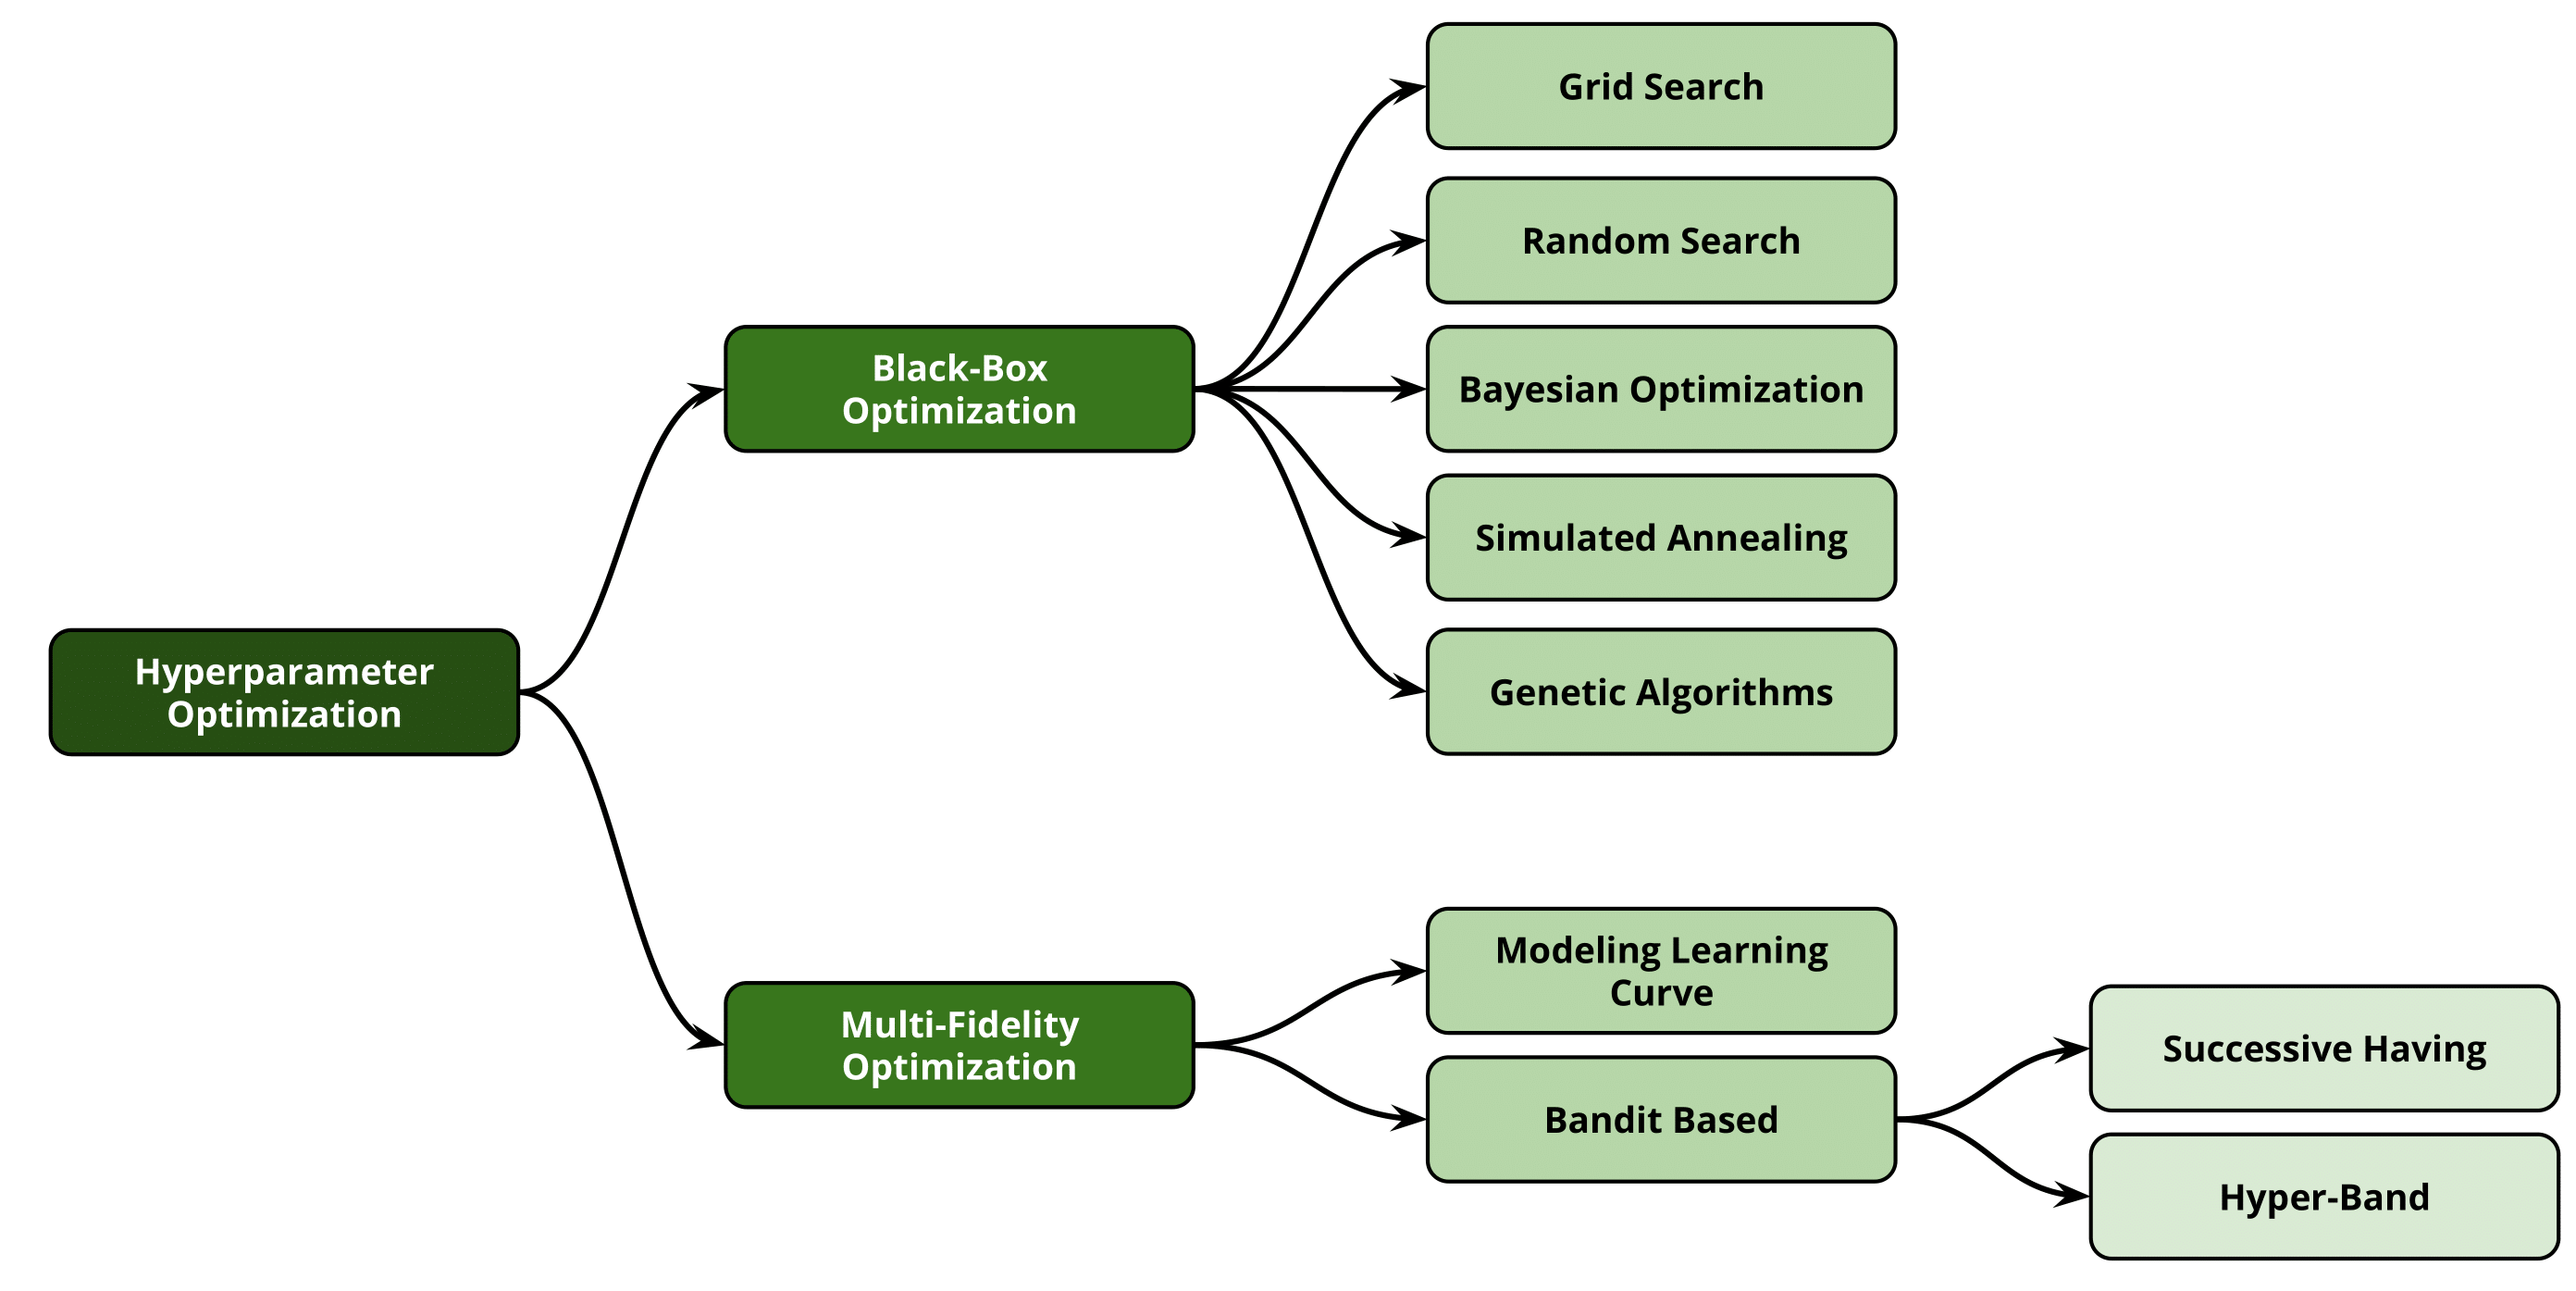
\includegraphics[width=0.75\textwidth]{images/state_art-taxonomy_optimizers.png}
	\caption{A Taxonomy for the Hyper-parameter Optimization Techniques \cite{elshawi2019automated}.}
	\label{fig:state_of_art_taxonomy}
\end{figure}

\subsection{Black Box Optimization Algorithms}

Black-box optimization algorithms treat the optimizable function a black-box (a process that is not analytically available) \cite[ch.~1]{book}. Therefore, any algorithm that does not directly infer any information from the optimizable function can be considered to be a black box algorithm.

\subsubsection{Grid Search and Random Search}

Traditionally grid search is used for HPO \cite{liashchynskyi2019grid}, where a researcher defines possible values for a given hyper parameter and tests every hyper parameter combination from the solution space provided (see Figure \ref{random}).

\begin{figure}[h]
	\centering
	\begin{subfigure}[t]{0.4\textwidth}
		\resizebox{\textwidth}{\textwidth}{%
			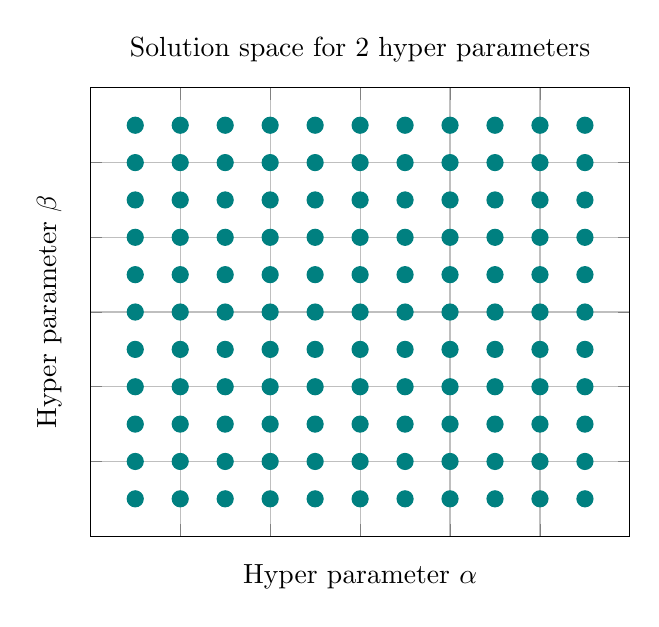
\begin{tikzpicture}
				\begin{axis}[
					title={Solution space for 2 hyper parameters},
				    xlabel={Hyper parameter $\alpha$},
				    ylabel={Hyper parameter $\beta$},
				    xmin=0, xmax=6,
				    ymin=0, ymax=6,
				    xtick={0,1,2,3,4,5},
				    ytick={0,1,2,3,4,5},
				    ymajorgrids=true,
				    xmajorgrids=true,
				    xticklabels={},
				    yticklabels={}
				]
				\addplot+[
					only marks,
				    mark options={color=teal},
				    mark=*,
				    mark size=2.9pt]
				    coordinates {
				    (0.5,0.5)(0.5,1)(0.5,1.5)(0.5,2)(0.5,2.5)(0.5,3)(0.5,3.5)(0.5,4)(0.5,4.5)(0.5,5)(0.5,5.5)
				    (1,0.5)(1,1)(1,1.5)(1,2)(1,2.5)(1,3)(1,3.5)(1,4)(1,4.5)(1,5)(1,5.5)
				    (1.5,0.5)(1.5,1)(1.5,1.5)(1.5,2)(1.5,2.5)(1.5,3)(1.5,3.5)(1.5,4)(1.5,4.5)(1.5,5)(1.5,5.5)
				    (2,0.5)(2,1)(2,1.5)(2,2)(2,2.5)(2,3)(2,3.5)(2,4)(2,4.5)(2,5)(2,5.5)
				    (2.5,0.5)(2.5,1)(2.5,1.5)(2.5,2)(2.5,2.5)(2.5,3)(2.5,3.5)(2.5,4)(2.5,4.5)(2.5,5)(2.5,5.5)
				    (3,0.5)(3,1)(3,1.5)(3,2)(3,2.5)(3,3)(3,3.5)(3,4)(3,4.5)(3,5)(3,5.5)
				    (3.5,0.5)(3.5,1)(3.5,1.5)(3.5,2)(3.5,2.5)(3.5,3)(3.5,3.5)(3.5,4)(3.5,4.5)(3.5,5)(3.5,5.5)
				    (4,0.5)(4,1)(4,1.5)(4,2)(4,2.5)(4,3)(4,3.5)(4,4)(4,4.5)(4,5)(4,5.5)
				    (4.5,0.5)(4.5,1)(4.5,1.5)(4.5,2)(4.5,2.5)(4.5,3)(4.5,3.5)(4.5,4)(4.5,4.5)(4.5,5)(4.5,5.5)
				    (5,0.5)(5,1)(5,1.5)(5,2)(5,2.5)(5,3)(5,3.5)(5,4)(5,4.5)(5,5)(5,5.5)
				    (5.5,0.5)(5.5,1)(5.5,1.5)(5.5,2)(5.5,2.5)(5.5,3)(5.5,3.5)(5.5,4)(5.5,4.5)(5.5,5)(5.5,5.5)
				    };
				\end{axis}
			\end{tikzpicture}
		}
	\end{subfigure}
	\begin{subfigure}[t]{0.4\textwidth}
		\resizebox{\textwidth}{\textwidth}{%
			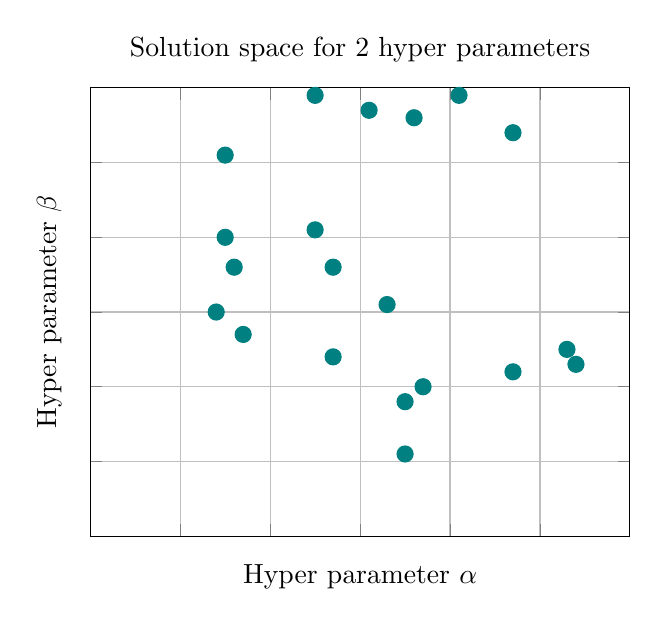
\begin{tikzpicture}
				\begin{axis}[
					title={Solution space for 2 hyper parameters},
				    xlabel={Hyper parameter $\alpha$},
				    ylabel={Hyper parameter $\beta$},
				    xmin=0, xmax=6,
				    ymin=0, ymax=6,
				    xtick={0,1,2,3,4,5},
				    ytick={0,1,2,3,4,5},
				    ymajorgrids=true,
				    xmajorgrids=true,
				    xticklabels={},
				    yticklabels={}
				]
				\addplot+[
					only marks,
				    mark options={color=teal},
				    mark=*,
				    mark size=2.9pt]
				    coordinates {
						(1.5,4)(2.5,4.1)(1.4,3)(1.6,3.6)(5.3,2.5)(5.4,2.3)(2.7,3.6)(1.5,5.1)(3.5,1.1)(3.1,5.7)(3.3,3.1)(3.5,1.8)(4.7,5.4)(3.7,2)(4.7,2.2)(2.7,2.4)(3.6,5.6)(2.5,5.9)(1.7,2.7)(4.1,5.9)
				    };
				\end{axis}
			\end{tikzpicture}
		}
	\end{subfigure}
    \caption{Illustration of a random search and a grid search.}
    \label{random}
\end{figure}

This method is similar to grid search, but replaces manually set values with ranges and allows for randomized selection of hyper parameter values (see Figure \ref{random}). This method has been proven to be more efficient than grid search \cite{JMLR:v13:bergstra12a}.

\subsubsection{Simulated Annealing}

This algorithm is based in the annealing process observed in metallurgy and it maintains a single candidate solution and takes steps of random size from the candidate in the search space, replacing the current candidate with a better solution or, with a certain probability, a worse one \cite{elshawi2019automated}.

\subsubsection{Bayesian Optimization}

Bayesian optimization can be described as sequential model-based optimization, whereas a probabilistic model is updated after every optimization attempt \cite{dewancker}.

Various probabilistic regression models can be used (e.g. Gaussian Processes and Random Forests).

\subsubsection{Genetic Algorithms}

This category of optimization methods use algorithms inspired by biological evolution.

These algorithms are usually based on the idea of applying the multiple genetic operations (crossover, mutation, survival of the fittest) to a population of configurations \cite{elshawi2019automated}.

\subsection{Multi-Fidelity Optimization Algorithms}

An area of increased attention in the HPO research field is multi-fidelity techniques. These methods focus on decreasing the evaluation cost of a given function by combining cheap low-fidelity and expensive high-fidelity evaluations \cite{elshawi2019automated}. These techniques are essential for optimization in high cost functions, where optimizing one hyper parameter can take days. These algorithms use more than a single model for estimating the optimizable parameters, whereas black box optimization algorithms use only one model.

\subsubsection{Bandit-based Optimization}

These techniques are based on the \textit{multi-armed bandit problem}, whereas a limited set of resources must be allocated between competing choices, maximizing expected gain \cite{Katehakis1987TheMB}. Similarly, using this class of algorithms in HPO allows computers to stop the execution of a trainable (with defined hyper parameter values), by analysing observable features during the run. This also leads to a decrease in computational power and time required to tune hyper parameters.

Examples of this category of algorithms are Successive Halving \cite{jamieson2015nonstochastic}, HyperBand \cite{li2016hyperband} and BOHB (Bayesian Optimization HyperBand) \cite{pmlr-v80-falkner18a}.

\subsubsection{Learning Curve Modelling}

Within more specific tasks, HPO can be performed by modelling the learning curve of a given function or network and using this model to extrapolate optimal hyper parameter values \cite{10555}. As this type of optimization is outside the scope of this project (seeing as it is meant to handle general functions), we do not investigate this optimization algorithm typology further.

\section{Software Interfaces}

In order to successfully integrate the HPO optimization framework with the pre-existing software, interfacing was required. To do this, a translation layer was developed between the framework's API and the pre-existing software's API. The framework required the development of a \textit{trainable}. Due to shortcomings in the pre-existing software infrastructure, these \textit{trainables} where obligatorily single-threaded.

\subsection{\textit{Trainable}}

Within the used framework, a unit of work was defined (the \textit{trainable}). This unit consists of a set of steps that are ran by the optimizer algorithm when testing a set of hyper parameter values.

First is the setup, where the framework performs any task that is required before executing the optimizable function (e.g. loading a file, validating system integrity, etc.).

Afterwards there is the step definition, where the framework performs the actual optimizable function. This is usually done as a stepped execution, allowing for pausing and terminating of trials. This means that, for the developed implementation, a set of scenarios where tested per trainable execution.

\subsection{Existing Software}

The pre-existing software (which contains the optimizable function) provides a plethora of internal APIs that can be used to trigger actions within (e.g. opening files, executing algorithms and others). Due to this, each step in the \textit{trainable} implementation consists of a variety of API calls.

\section{Data Visualization}

\section{Results}

\bibliographystyle{splncs04}
\bibliography{refs}

\end{document}